\documentclass[UTF8,a4paper,zihao=-4,fontset=none]{ctexart}
\usepackage[margin=2.2cm]{geometry}
\usepackage{amsmath,amssymb,graphicx,longtable,array,booktabs,url}
\usepackage{float}
\usepackage[hidelinks]{hyperref}
\setCJKmainfont{Noto Serif CJK SC}
\setCJKsansfont{Noto Sans CJK SC}
\setCJKmonofont{Noto Sans Mono CJK SC}
\setlength{\emergencystretch}{2em}
\setlength{\LTpre}{0.5em}
\setlength{\LTpost}{0.5em}
\begin{document}
\section{问题一：多模态特征提取与时序对齐}
% 独立配图版：宋体与Times New Roman配图，独立PDF通过minipage排列。
% 本文件统一包含结果分析、全量汇总和复现说明；只需input本文件一次。
% 依赖 graphicx、float、longtable、array、booktabs、url；配套表格与results_delivery.tex置于同目录。
\subsection{实验结果分析}
\label{sec:p1_results}
\newsavebox{\pOneResultTableBox}
% 文件名与样本编号随正文排字，同时保留特殊字符处理及换行能力。
\urlstyle{same}

前文建立了以词为单位的三模态特征表示，并分别记录了观测有效性与词级对齐信息。在此基础上，本节考察特征提取的覆盖情况、词级时间对应的质量及不同时间粒度对特征表示的影响，结合人工审核解释异常原因，并通过典型样本检验词与原始视听记录之间的映射，最后汇总全部样本的输出结果。实验采用固定参数的预训练模型，不涉及情感预测模型的训练，因此主要评价特征提取与时序组织的结果。

\subsubsection{样本覆盖完整性与特征有效性}
\label{sec:p1_quality_scope}

按照前文的词级聚合方法，100条样本均生成了文本、声学和视觉特征矩阵。各样本的矩阵行数与原文词数一致，三种模态均与原始转写中的1932个词逐一对应，未出现词序列截断。表~\ref{tab:p1_result_overview}给出了样本处理与模态观测的覆盖情况。

\begin{table}[H]
    \centering\small
    \caption{样本处理与三种模态的观测覆盖情况}
    \label{tab:p1_result_overview}
    \renewcommand{\arraystretch}{1.18}
    \begin{lrbox}{\pOneResultTableBox}
\begin{tabular}{@{}lrr@{}}
        \hline
        统计项目 & 数量 & 占比\\ \hline
        已处理样本 & 100 & 100.00\%\\
        与原文对应的输出词位置 & 1932 & 100.00\%\\
        文本模态可观测的词 & 1932 & 100.00\%\\
        声学模态可观测的词 & 1932 & 100.00\%\\
        视觉模态可观测的词 & 1595 & 82.56\%\\
        \hline
    \end{tabular}
\end{lrbox}
\usebox{\pOneResultTableBox}
    \par\smallskip
    \parbox{\wd\pOneResultTableBox}{\footnotesize 注：样本比例以100为分母，词比例以1932为分母，各行不是互斥类别。观测覆盖表示相应位置存在可用于特征计算的记录。}
\end{table}

沿用前文对有效观测的定义，某词的某一模态“可观测”，是指该位置具有文本表示，或存在与其候选时间区间交叠、可参与聚合的有效声学或面部记录。全量共得到77261条声学记录和3973帧抽样画面，其中3253帧成功提取面部特征，720帧未获得可用结果，占18.12\%。经词级聚合，1595个词的视觉模态可观测，占82.56\%；其余337个词没有对应的有效面部记录。因此，三种模态的矩阵行数虽然相同，各词位置的观测完整性仍存在差异。由于一个词可以关联多帧，一帧也可能参与多个词的聚合，帧级与词级的缺失比例并不相同。

图~\ref{fig:p1_observation_work}至图~\ref{fig:p1_observation_similar}展示了上述差异的具体表现。在样本-s9qJ7ATP7w\$\_\$7中，work对应的两帧均未获得面部特征，因而该词的视觉特征采用零向量占位；同一样本的day对应两帧有效面部记录，可以形成视觉表示。样本-iRBcNs9oI8\$\_\$9中的similar对应画面虽有人物，仍未获得可用面部特征，说明观测缺失不能直接归因于画面无人。三图分别展示0.8000、4.0000、1.6016 s处的实际画面；下方依次给出帧代表区间与候选词区间，绿色和灰色分别表示面部观测有效与无效。帧代表区间采用前文所述的相邻抽样时刻中点划分方式。

\begin{figure}[H]
    \centering
    \begin{minipage}[t]{.32\linewidth}
        \vspace{0pt}
        \centering
        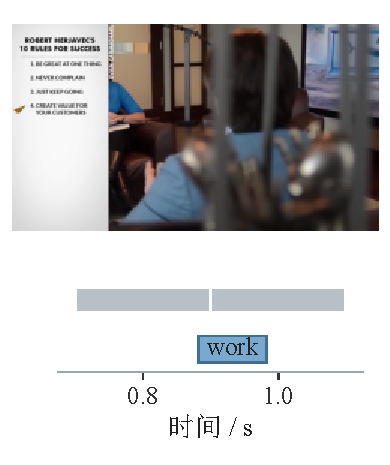
\includegraphics[width=\linewidth]{figures/fig_p1_observation_work.pdf}
        \caption{work的面部观测}
        \label{fig:p1_observation_work}
    \end{minipage}\hfill
    \begin{minipage}[t]{.32\linewidth}
        \vspace{0pt}
        \centering
        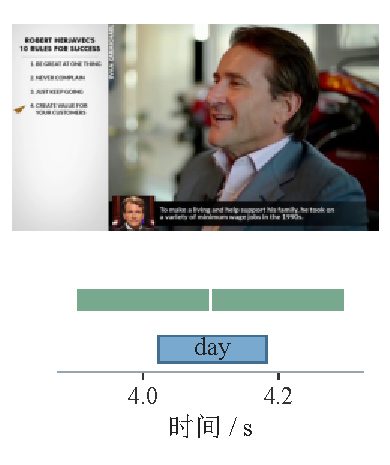
\includegraphics[width=\linewidth]{figures/fig_p1_observation_day.pdf}
        \caption{day的面部观测}
        \label{fig:p1_observation_day}
    \end{minipage}\hfill
    \begin{minipage}[t]{.32\linewidth}
        \vspace{0pt}
        \centering
        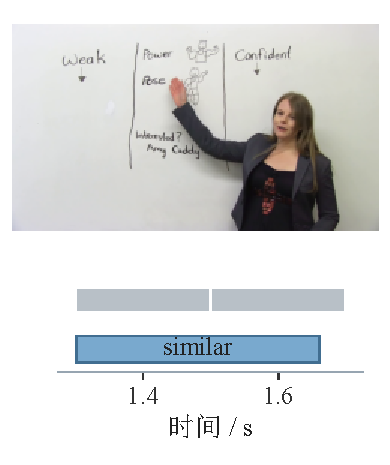
\includegraphics[width=\linewidth]{figures/fig_p1_observation_similar.pdf}
        \caption{similar的面部观测}
        \label{fig:p1_observation_similar}
    \end{minipage}
\end{figure}

声学模态虽然在全部词位置均有可计算记录，但其信号强度存在差异。为识别幅度较低的输入，以数字音频满幅1为基准，将短时均方根幅度（RMS）低于0.0031623的记录标记为低能量，共9918条，占12.84\%。低能量表示该短时记录的波形幅度较小，不等同于观测缺失，也不能直接判定该区间没有语音。图~\ref{fig:p1_visual_coverage}汇总了面部特征的帧级与词级覆盖情况，图~\ref{fig:p1_audio_energy_share}则给出了低能量声学记录的占比。两图分别反映面部特征能否提取与音频信号幅度，统计含义不同。

\begin{figure}[H]
    \centering
    \begin{minipage}[t]{.48\linewidth}
        \vspace{0pt}
        \centering
        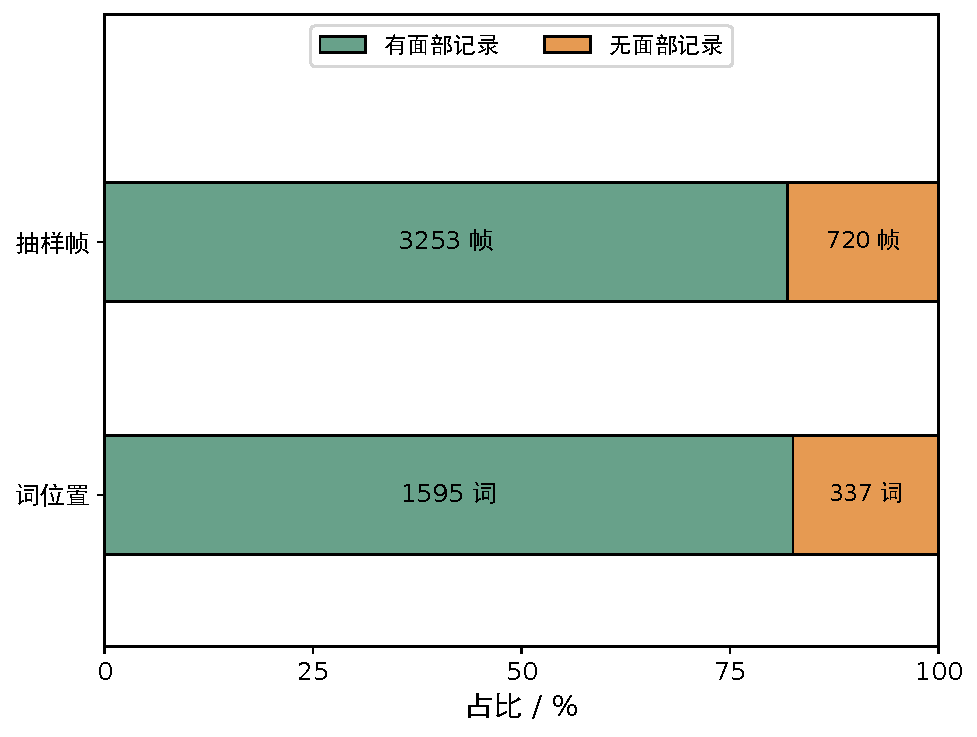
\includegraphics[width=\linewidth]{figures/fig_p1_visual_coverage.pdf}
        \caption{面部特征的帧级与词级覆盖}
        \label{fig:p1_visual_coverage}
    \end{minipage}\hfill
    \begin{minipage}[t]{.48\linewidth}
        \vspace{0pt}
        \centering
        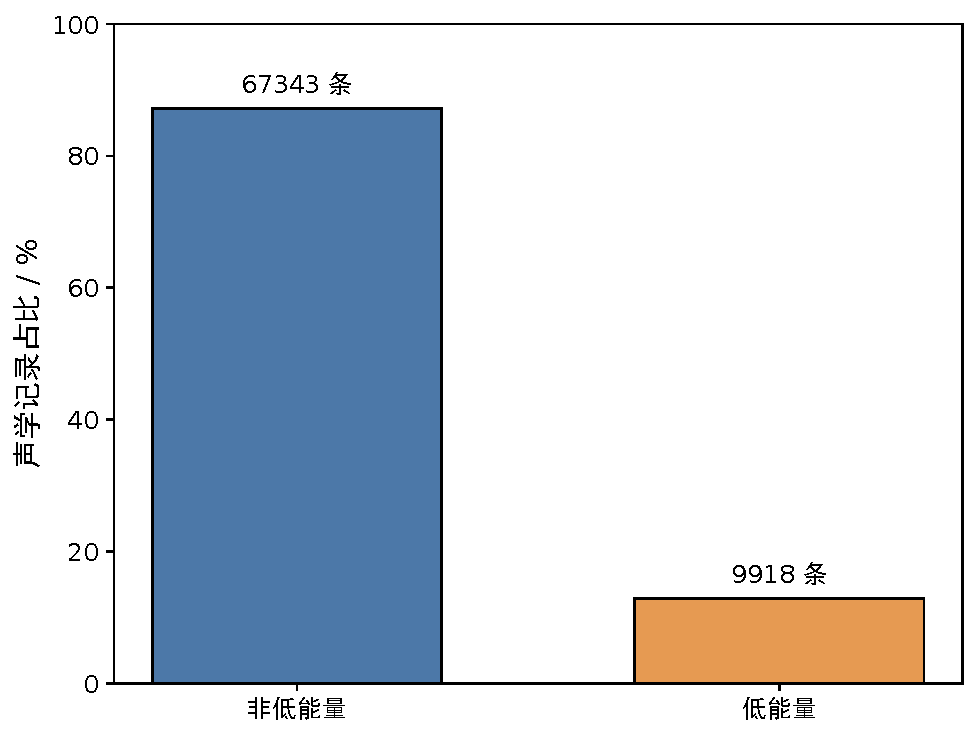
\includegraphics[width=\linewidth]{figures/fig_p1_audio_energy_share.pdf}
        \caption{声学记录的低能量占比}
        \label{fig:p1_audio_energy_share}
    \end{minipage}
\end{figure}

以样本-iRBcNs9oI8\$\_\$9为例，其333条声学记录中有147条属于低能量记录。图~\ref{fig:p1_rms}展示完整的RMS变化，图~\ref{fig:p1_rms_zoom}放大同一数据的低幅值范围；虚线表示阈值，橙点表示低能量记录。低幅区间仍能计算声学特征，因此不能将低能量记录作为缺失值处理。此外，有两条样本的解码音频波形全为零，其声学特征各维均不随时间变化。这说明声学特征的数值覆盖完整，并不意味着每条样本都包含有效语音；后文将进一步检查这两条样本对时间粒度对照结果的影响。

\begin{figure}[H]
    \centering
    \begin{minipage}[t]{.48\linewidth}
        \vspace{0pt}
        \centering
        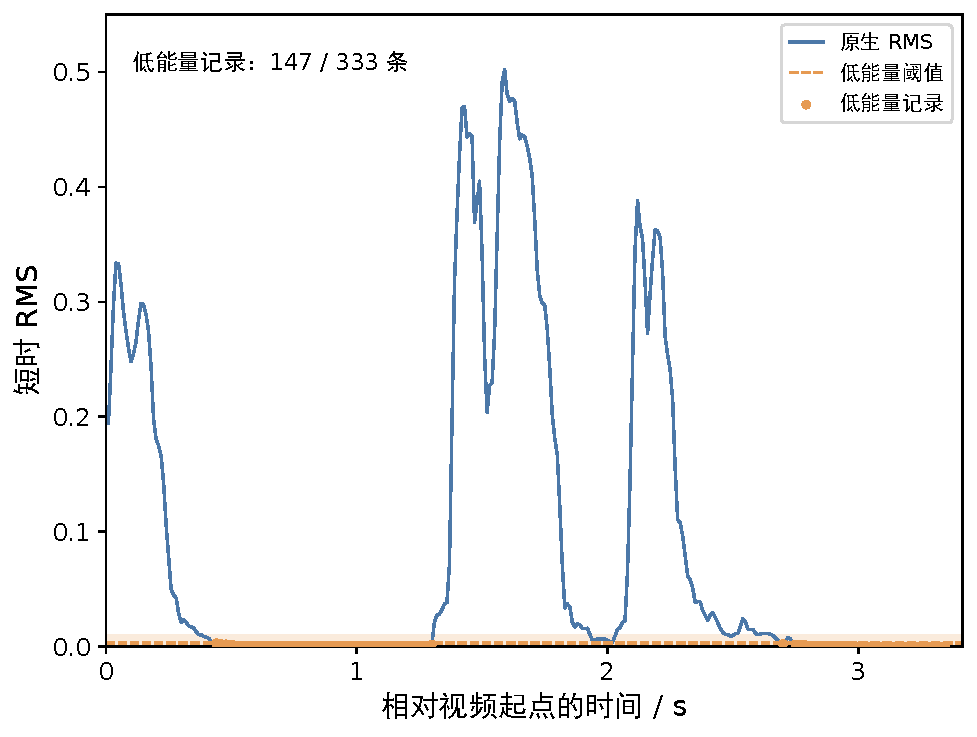
\includegraphics[width=\linewidth]{figures/fig_p1_rms.pdf}
        \caption{实例音频的短时RMS}
        \label{fig:p1_rms}
    \end{minipage}\hfill
    \begin{minipage}[t]{.48\linewidth}
        \vspace{0pt}
        \centering
        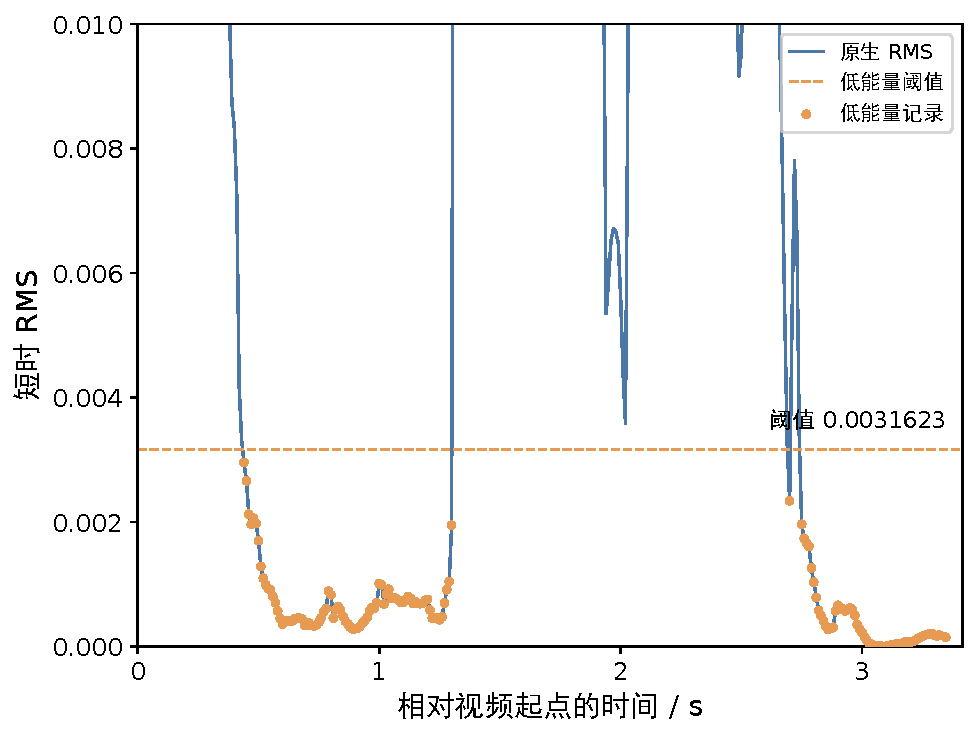
\includegraphics[width=\linewidth]{figures/fig_p1_rms_zoom.pdf}
        \caption{短时RMS的低幅值范围}
        \label{fig:p1_rms_zoom}
    \end{minipage}
\end{figure}

\subsubsection{时序对齐质量评估与人工审核}
\label{sec:p1_timing_quality}

前文的CTC强制对齐为1932个词均生成了候选时间区间，但路径满足给定转写的字符约束，并不意味着词界定位准确。为评价音频对候选对应关系的支持程度，本文进一步分析词级置信度与片段级转写一致性。词级置信度取最优CTC路径中属于该词的文字字符帧概率的几何平均，不包含空白符和词界符；分数较低，表示模型对这些字符在相应时刻出现的支持较弱。片段级指标采用诊断词错误率（Word Error Rate，WER），即不受给定转写约束的贪心识别文本与规范化转写之间的最少词编辑数除以参考词数。两项指标分别考察局部字符匹配与整段文本差异，均基于同一声学模型，不构成相互独立的准确性验证。

如图~\ref{fig:p1_ctc_confidence}所示，词级置信度的均值为0.7477，中位数为0.9585，1034个词的分数不低于0.95，但仍有350个词低于0.1，占18.12\%。高分词较多的同时仍存在一批低分词，说明仅依据整体均值或中位数，难以识别局部对齐异常。图~\ref{fig:p1_diagnostic_wer}中，诊断WER的均值为0.4689，21条样本超过0.8，其中9条超过1。由于编辑数包含插入操作，WER可以大于1。两图虚线分别标示0.1和0.8；统计对象分别为1932个词与100条样本。需要说明的是，CTC置信度未经人工词界标注校准，诊断WER也可能受到自动识别错误的影响，因此二者用于发现待复核结果，不能直接解释为对齐准确率或真实词界误差。

\begin{figure}[H]
    \centering
    \begin{minipage}[t]{.48\linewidth}
        \vspace{0pt}
        \centering
        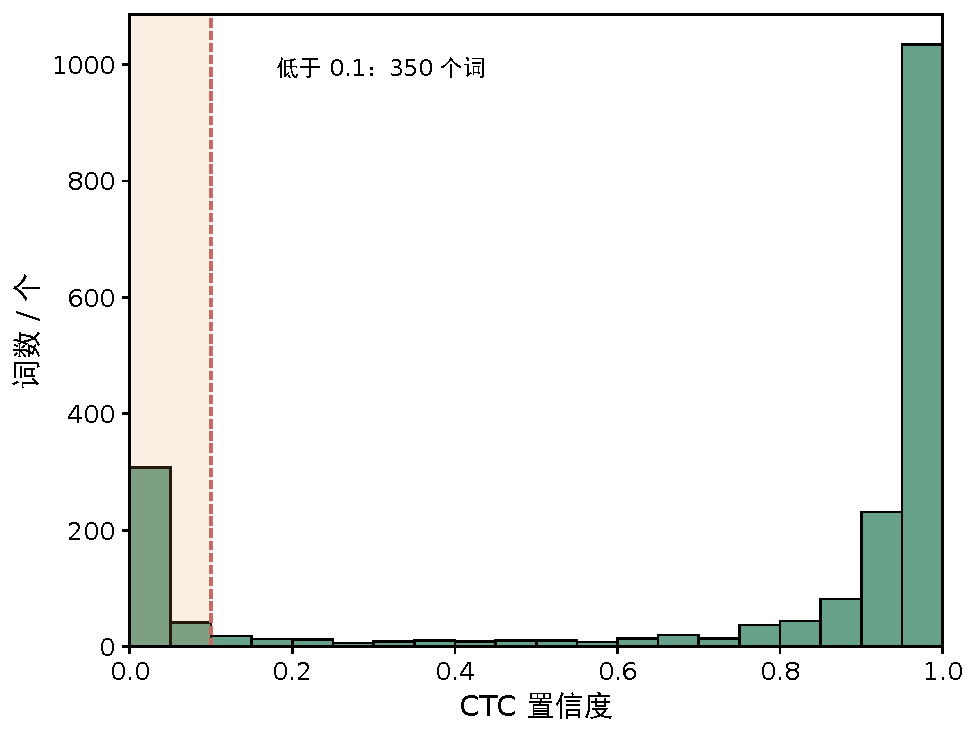
\includegraphics[width=\linewidth]{figures/fig_p1_ctc_confidence.pdf}
        \caption{词级CTC置信度分布}
        \label{fig:p1_ctc_confidence}
    \end{minipage}\hfill
    \begin{minipage}[t]{.48\linewidth}
        \vspace{0pt}
        \centering
        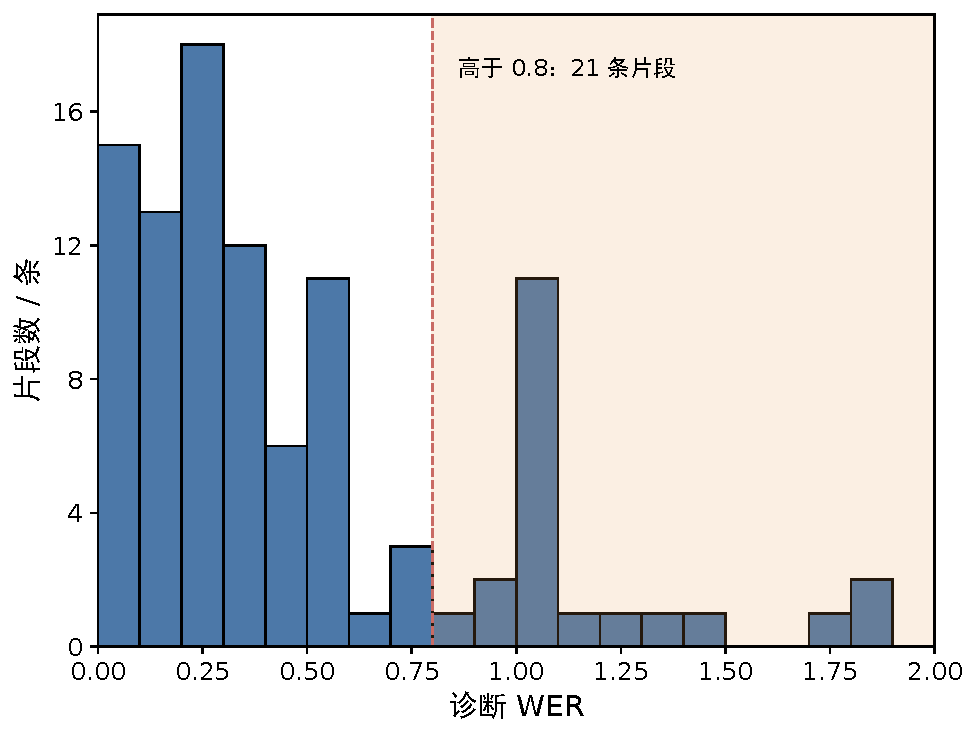
\includegraphics[width=\linewidth]{figures/fig_p1_diagnostic_wer.pdf}
        \caption{片段级诊断WER分布}
        \label{fig:p1_diagnostic_wer}
    \end{minipage}
\end{figure}

以样本-iRBcNs9oI8\$\_\$9为例，给定转写为Power is similar to strength，识别结果为OF POWER EPOSE，诊断WER为1.0000，5个词的平均置信度仅0.000385。结合前述面部观测缺失，该样本同时存在模态缺失和转写一致性风险，不宜直接用于词级三模态对应分析。

为区分可用于后续词级分析的结果与需要复核的结果，本文实施两层对齐质量筛选。首先，在片段层面，将平均词置信度低于0.2、置信度低于0.1的词超过一半、诊断WER大于0.8或无法形成完整CTC路径的样本列入复核，暂不采用其词级时间对应。其次，在其余样本中，仅将成功获得候选起止时间且置信度不低于0.1的词计为通过筛选。上述处理只增加质量标记，不删除原文词、特征向量或候选时间记录。阈值是在检查实际异常后设定的保守筛选条件，未利用情感标签或人工词界标注进行优化。

按上述条件，四项片段级筛选分别标记19、20、21和0条样本，前三项标记集合均包含在诊断WER大于0.8的样本集合中，最终共有21条样本需要整段复核。这些样本包含317个词，其余79条样本中另有70个词因置信度不足而未通过筛选。因此，1932个词中有1545个通过对齐质量筛选，占79.97\%。其中，1387个词的三种模态都可观测，占全部词的71.79\%；另外158个词缺少有效面部记录。未通过筛选的387个词多于低置信度词的350个，是因为片段级复核还涉及其中37个局部置信度达到阈值的词。由此可见，词级跨模态分析既需要相应模态可观测，也需要检查该词及所在片段的对齐质量。

为考察筛选结果对阈值的依赖，将片段平均置信度阈值分别取0.1、0.2、0.3，诊断WER阈值分别取0.6、0.8、1.0，其余条件不变。在三种平均置信度阈值下，待复核样本数均随WER阈值变化依次为25、21、20条，说明当前数据的筛选数量主要受WER条件影响。该对照反映了复核范围对阈值的敏感性；由于缺少人工词界标注，尚不能据此确定最优阈值。

自动诊断能够提示潜在异常，但难以区分低分究竟来自语音内容差异、输入语言不匹配，还是音频本身缺少对应朗读。因此，在自动筛选之后，对上述21条样本进行人工审核，对照实际音频与给定英文转写，检查片段内容是否对应。审核结果按主要问题归为五类，见表~\ref{tab:p1_manual_review}，各类互不重叠，共涉及317个原文词。

% 用户提供的人工审核结果；由build_manual_review.py汇总。
\begin{table}[H]
    \centering\small
    \caption{21条复核样本的人工审核结果}
    \label{tab:p1_manual_review}
    \setlength{\tabcolsep}{5pt}
    \renewcommand{\arraystretch}{1.2}
    \begin{tabular}{@{}lrr>{\raggedright\arraybackslash}p{5.0cm}@{}}
        \toprule
        审核发现 & 样本数 & 原文词数 & 主要表现\\ \midrule
        音轨与文本不对应 & 11 & 120 & 实际语音内容与给定转写不对应。\\
        无对应朗读 & 5 & 64 & 未听到对应朗读，其中1条为音乐。\\
        非英语语音 & 3 & 93 & 实际语音并非英语。\\
        分段内容不对应 & 1 & 18 & 前半段无朗读，后半段语音与转写不对应。\\
        音频卡顿、局部对应 & 1 & 22 & 音频存在卡顿，部分词语与文本一致，但未形成完整对应。\\
        \midrule
        合计 & 21 & 317 & \\
        \bottomrule
    \end{tabular}
\end{table}


其中，11条样本的语音内容与给定转写不对应；5条未听到对应朗读，包括1条音乐片段及前述解码波形全为零的两条样本。另有1条样本前半段无朗读、后半段语音与文本不对应，单独归为分段内容不对应。3条非英语语音均来自视频-yRb-Jum7EQ，与本文采用的英语字符识别模型及英文对齐目标不匹配。因此，这些样本的低置信度或较高诊断WER具有不同来源，不能统一解释为词界定位偏差。

样本-HwX2H8Z4hY\$\_\$9体现了另一种情况：人工审核发现原始音频存在卡顿，部分词语与给定文本一致，但整体内容并非逐词对应。该样本平均词置信度为0.7238，仅9.09\%的词低于0.1，却因诊断WER达到0.8636而进入复核范围。这表明，局部词语能够匹配并不足以确认整段对应关系，也说明片段级文本一致性检查在发现此类异常中的作用。

人工审核为这21条样本补充了具体的异常解释，因而继续将其整体词级对应标记为受限，并保存原文、候选时间与原生视听特征。本次审核未进一步重建词级时间边界，故不据此恢复个别词的对齐标记，前述1545个通过筛选的词及其中1387个三种模态都可观测的词的统计保持不变。本次人工审核仅覆盖自动筛出的21条样本，不能据此认定其余79条样本均无异常，也不能计算全量词界准确率。逐样本审核说明随结果附件保存。

\label{sec:p1_window_analysis}

上述分析考察了候选词区间与实际语音内容的对应质量。在此基础上，为进一步考察时间划分对特征表示的影响，在相同原生特征上构造0.2 s和0.5 s两种固定窗口，共形成200条对照记录。窗口从零时刻开始，末窗截取至片段终点，视听特征仍按前文的时间交叠方法聚合。对照关注两个方面：将窗口特征映回原生记录，以各维原生标准差归一化后的重建均方误差衡量原生特征变化的保留程度；在通过对齐质量筛选的词中，统计与两个及以上窗口交叠的词比例，考察词区间被窗口边界切分的频率。两项指标均先在样本内计算，再对相应有效样本等权平均。

以第~\ref{sec:p1_verification_examples}~节所展示的典型样本为例，图~\ref{fig:p1_window_reconstruction}显示，窗口平均削弱了原生响度的局部峰谷，较长窗口的平滑范围更大。图~\ref{fig:p1_word_window_overlap}中，绿色线为successful区间，着色格为与其交叠的窗口；该词分别与4个短窗、2个长窗交叠。该例说明，更细的划分有利于保留局部变化，但也引入了更多可能切分词区间的边界。跨界比例仅判断是否被切分，不区分微小越界与大幅切分。该词终点约为2.40247 s，与第四个短窗仍有约0.00247 s的交叠，故计入跨界；每个词只计一次，计算以大于$10^{-8}\,\mathrm{s}$的交叠排除数值误差。

\begin{figure}[H]
    \centering
    \begin{minipage}[t]{.48\linewidth}
        \vspace{0pt}
        \centering
        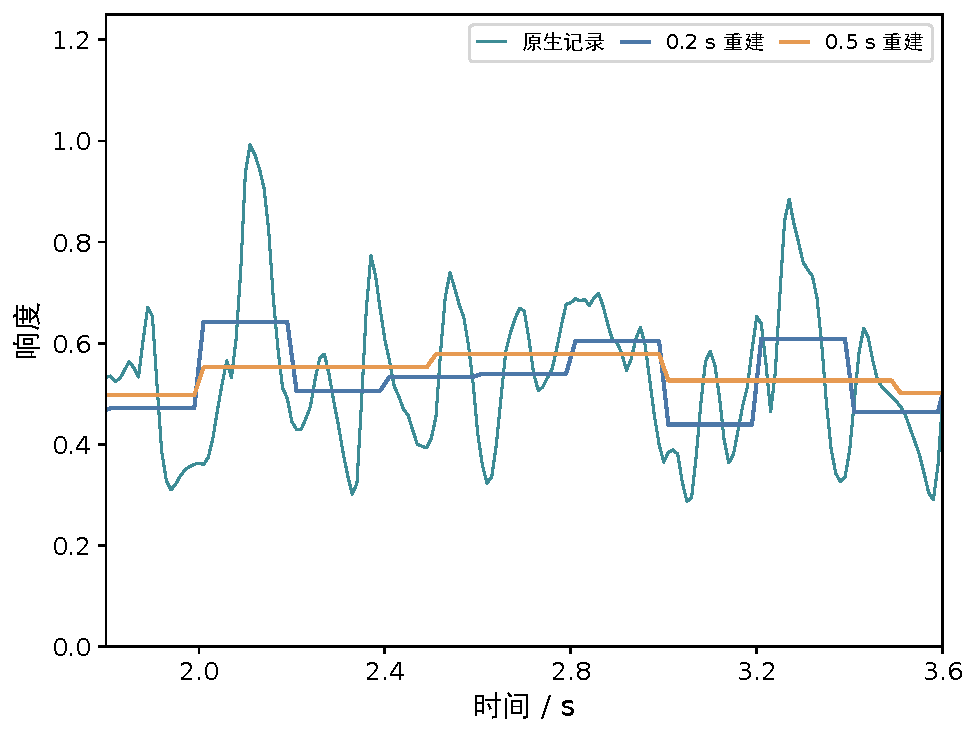
\includegraphics[width=\linewidth]{figures/fig_p1_window_reconstruction.pdf}
        \caption{响度的固定窗聚合与重建}
        \label{fig:p1_window_reconstruction}
    \end{minipage}\hfill
    \begin{minipage}[t]{.48\linewidth}
        \vspace{0pt}
        \centering
        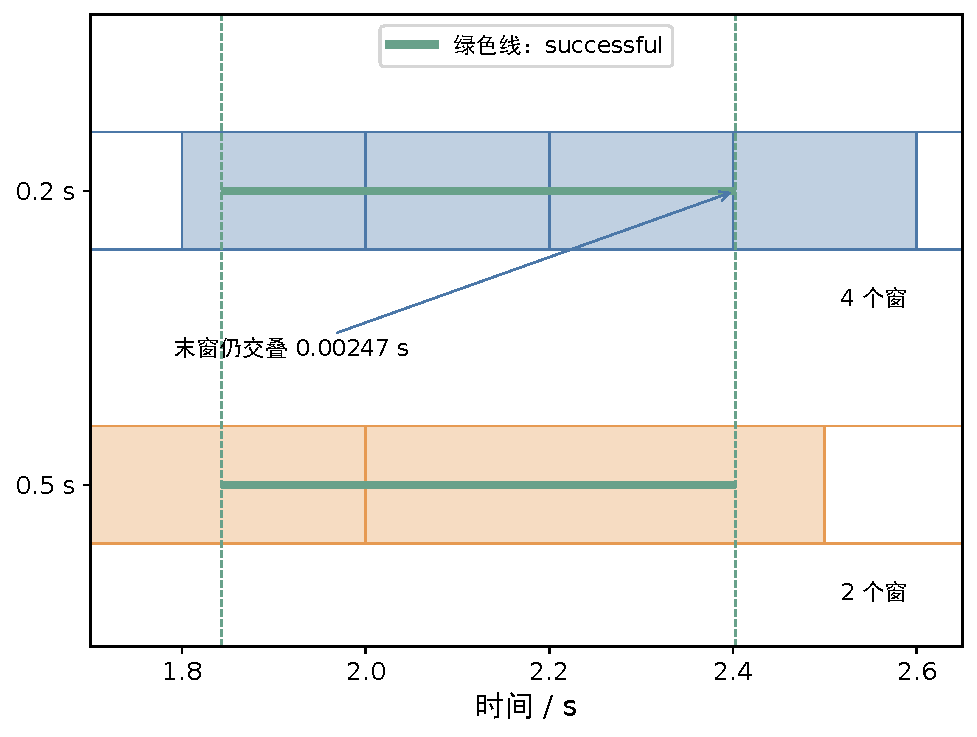
\includegraphics[width=\linewidth]{figures/fig_p1_word_window_overlap.pdf}
        \caption{候选词区间与固定窗口交叠}
        \label{fig:p1_word_window_overlap}
    \end{minipage}
\end{figure}

全量结果见图~\ref{fig:p1_audio_window_error}至图~\ref{fig:p1_word_crossing_ratio}。窗口由0.5 s缩短至0.2 s后，声学、视觉平均标准化重建误差分别由0.7467、0.4373降至0.5449、0.2357，相对降幅分别为27.02\%和46.10\%；平均词跨界比例则由39.50\%升至71.33\%，增加31.83个百分点。声学误差基于100条样本；13条样本无有效面部记录，视觉误差基于87条；21条样本被列入整段对齐复核，跨界比例基于其余79条。跨界比例的总体均值按样本等权计算，不是将全部词合并后的比例。

\begin{figure}[H]
    \centering
    \begin{minipage}[t]{.32\linewidth}
        \vspace{0pt}
        \centering
        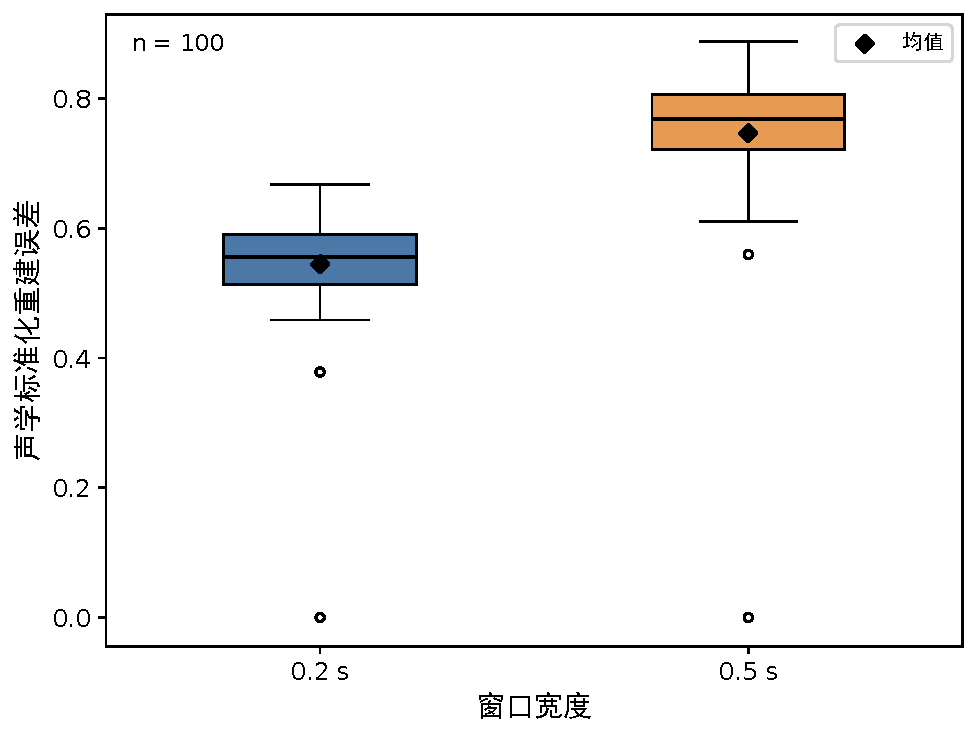
\includegraphics[width=\linewidth]{figures/fig_p1_audio_window_error.pdf}
        \caption{声学重建误差}
        \label{fig:p1_audio_window_error}
    \end{minipage}\hfill
    \begin{minipage}[t]{.32\linewidth}
        \vspace{0pt}
        \centering
        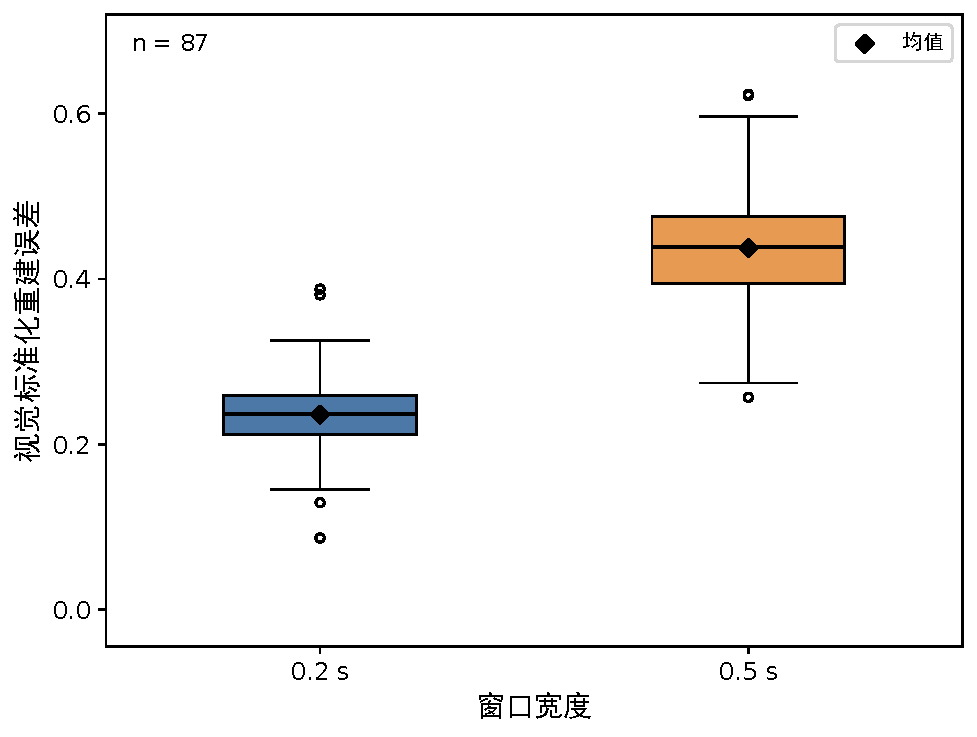
\includegraphics[width=\linewidth]{figures/fig_p1_vision_window_error.pdf}
        \caption{视觉重建误差}
        \label{fig:p1_vision_window_error}
    \end{minipage}\hfill
    \begin{minipage}[t]{.32\linewidth}
        \vspace{0pt}
        \centering
        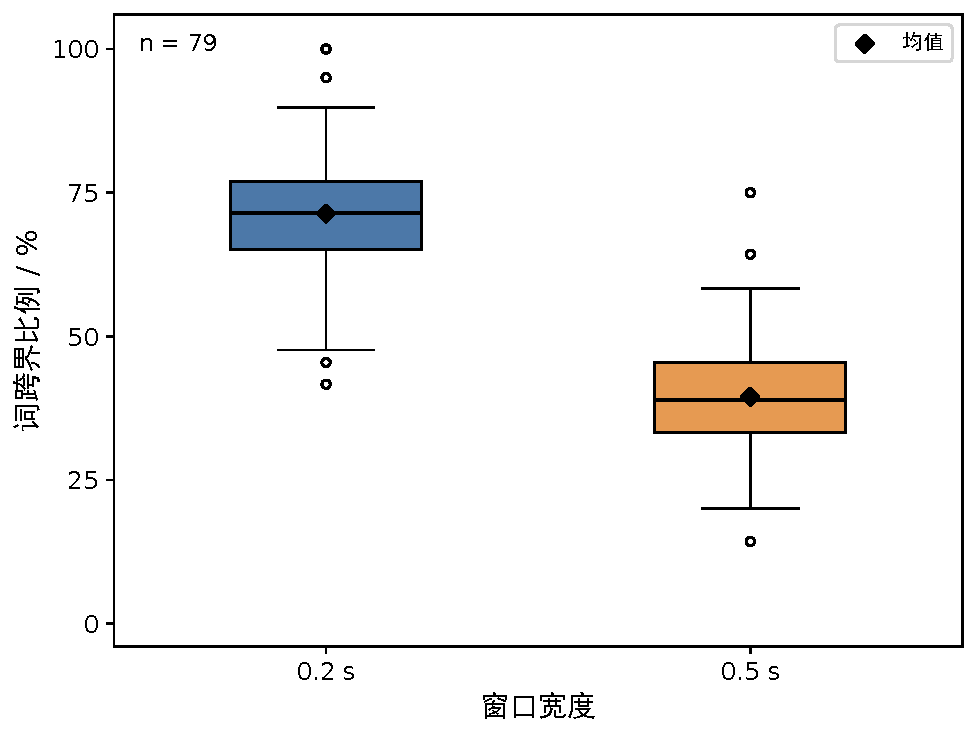
\includegraphics[width=\linewidth]{figures/fig_p1_word_crossing_ratio.pdf}
        \caption{词跨界比例}
        \label{fig:p1_word_crossing_ratio}
    \end{minipage}
\end{figure}

箱线图中，箱体为第25至第75百分位数，中线为中位数，须线延伸至1.5倍四分位距内的最远观测，须线外圆点仍参与统计，菱形为样本均值。重建误差仅纳入标准差大于$10^{-6}$的维度；有记录但全部维度恒定时记0，无有效记录时不计入模态均值。

对同一样本逐一比较，98条样本的短窗声学误差更低，另2条相同；87条样本的短窗视觉误差均更低；77条样本的短窗跨界比例更高，另2条相同。两条声学误差相同的样本即前述退化输入，其原生描述量无时间变化，两种窗口误差均按规则记0，故声学误差图每组的两个零值重叠。将这两条单独列出后，其余98条样本的0.2 s、0.5 s平均声学误差分别为0.5560和0.7619，差异方向保持一致。因此，短窗降低重建误差的结论并非由退化样本造成，零误差本身也不能解释为更充分的声音信息。

上述结果表明，较短窗口能够保留更多原生特征变化，但也更容易将同一词对应的视听信息分散到多个窗口。这与前文以词为基本对齐单位的考虑一致：词级表示便于按语义单元组织多模态信息，固定窗口则适用于不依赖词界的视听分析。该实验仅比较了两种固定窗口，不能据此断言词级表示具有更低的重建误差或更高的情感预测性能。

\subsubsection{典型样本的跨模态时序对齐验证}
\label{sec:p1_verification_examples}

为检验词级输出与原始记录之间的对应关系，在未触发整段复核且面部观测帧占比不低于80\%的样本中，选取时长最接近10 s的-egA8-b7-3M\$\_\$1进行展示。该样本时长10.266 s，含20个词，其中18个通过上述对齐质量筛选。

图~\ref{fig:p1_multimodal_result}给出了1.80--3.60 s内的局部对应。successful区间内约2.11 s处出现响度峰值；张嘴系数在2.8 s附近较大，随后降低，而左嘴角上扬系数整体较小。声学与面部特征分别记录声音和面部运动的变化，共同时间轴使这些变化能够回溯至相应词区间及实际画面。单项系数的高低不直接对应情感类别，实际计算得到的近零系数也不同于缺失后的零占位。图中各行共用时间轴，虚线表示候选词界；上方展示部分抽样帧，图像宽度不表示持续时间。响度取自openSMILE，与波形RMS不同；面部曲线连线仅辅助观察，不表示帧间连续实测。

\begin{figure}[H]
    \centering
    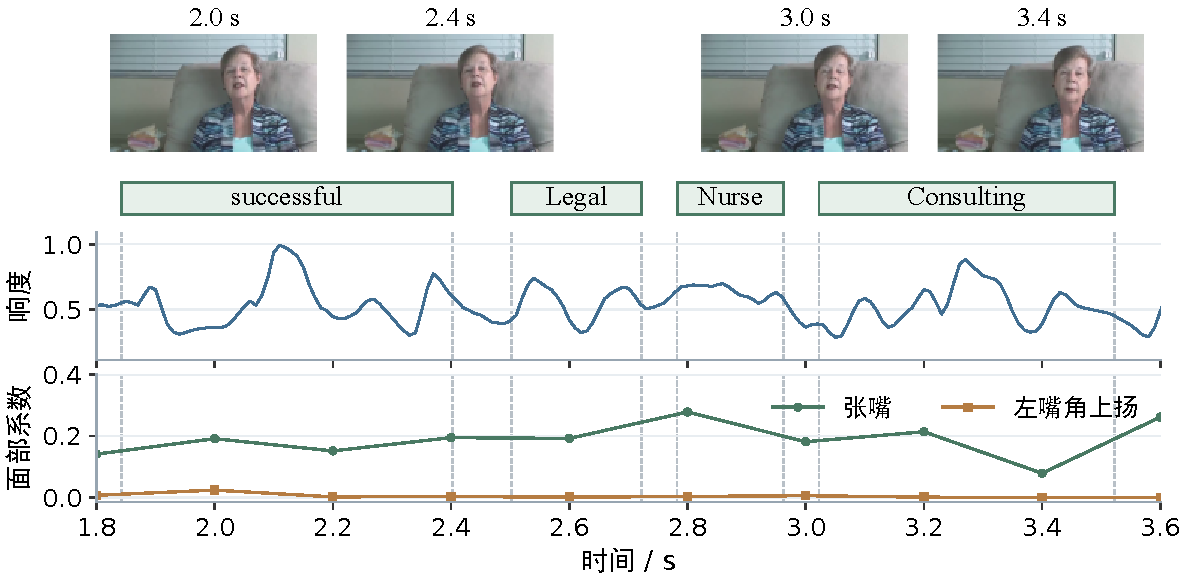
\includegraphics[width=0.94\linewidth]{figures/fig_p1_multimodal_timeline.pdf}
    \caption{典型样本的词区间与视听记录对应}
    \label{fig:p1_multimodal_result}
\end{figure}

表~\ref{tab:p1_mapping_records}列出部分映射记录。以successful为例，候选区间为$[1.8425,2.4025]\,\mathrm{s}$，其文本表示对应子词索引3，声学表示由183--240号共58条短时记录聚合，视觉表示由1.8、2.0、2.2、2.4 s四帧聚合。依据前文的时间交叠加权方法，边界帧仅部分覆盖词区间，其聚合权重相应较小。这一实例表明，词级向量能够对应到具体的子词、声学记录和视频帧，并可由保存的权重复算。

% 自动读取既有特征文件生成；由 results_section.tex 插入。
\begin{table}[H]
    \centering
    \caption{典型样本的部分词级映射记录}
    \label{tab:p1_mapping_records}
    \begingroup
    \small
    \setlength{\tabcolsep}{3pt}
    \renewcommand{\arraystretch}{1.2}
    \begin{lrbox}{\pOneResultTableBox}
\begin{tabular}{@{}l c c c l@{}}
        \hline
        原文词 & 子词索引 & 候选区间/s & 声学记录索引 & 视觉帧时刻/s\\ \hline
        started & 1 & $[1.2825,1.6425]$ & 127--164 & 1.2, 1.4, 1.6\\
        successful & 3 & $[1.8425,2.4025]$ & 183--240 & 1.8, 2.0, 2.2, 2.4\\
        Consulting & 6 & $[3.0225,3.5225]$ & 301--352 & 3.0, 3.2, 3.4, 3.6\\
        \hline
    \end{tabular}
\end{lrbox}
\usebox{\pOneResultTableBox}
    \par\smallskip
    \parbox{\wd\pOneResultTableBox}{\footnotesize 注：索引从0开始；声学索引指具有正聚合权重的原生特征记录，不是波形采样点。视觉帧按其时间支持区间与候选词区间的交叠关系参与聚合，帧中心不必位于词区间内部。}
    \endgroup
\end{table}


在实例展示之外，对全部词的交叠权重、视听聚合值和CTC置信度进行独立复算，并重新计算诊断WER、解码音视频核对时间记录与低能量标记，100条样本均与保存结果一致。这说明输出符合既定计算方法。典型样本中的in和1989仍因置信度不足而未通过逐词筛选，表明片段整体未被列入复核，并不排除局部异常。上述计算核验验证的是结果与计算规则的一致性，词界的实际定位误差仍需人工标注后评价。

% 下列文件为本小节的组成部分，无单独的subsection。
% 本文件由results_section.tex末尾调用，属于同一个“实验结果分析”小节。
% 依赖 longtable、array、booktabs、url。
\subsubsection{三模态特征文件说明与100条样本结果汇总}
\label{sec:p1_delivery}

上述分析分别给出了模态观测情况与对齐质量的统计结果。为进一步呈现各样本之间的差异，表~\ref{tab:p1_all_samples}按原样本编号汇总全部100条样本的输出。三种模态的共同规格见表~\ref{tab:p1_feature_specification}，全量表则列出各样本的时长、原文词数、视觉可观测词数及通过对齐质量筛选的词数。两表共同说明输出特征的维数、长度与有效位置，高维特征的具体数值另存于对应文件中。

\begin{table}[H]
    \centering\small
    \caption{三种模态的词级特征规格}
    \label{tab:p1_feature_specification}
    \renewcommand{\arraystretch}{1.18}
    \begin{lrbox}{\pOneResultTableBox}
\begin{tabular}{@{}lccc@{}}
        \toprule
        模态 & 特征维数 & 样本矩阵形状 & 对齐粒度\\ \midrule
        文本 & 768 & $L\times768$ & 原文词\\
        声学 & 25 & $L\times25$ & 原文词\\
        视觉（面部） & 52 & $L\times52$ & 原文词\\ \bottomrule
    \end{tabular}
\end{lrbox}
\usebox{\pOneResultTableBox}
    \par\smallskip
    \parbox{\wd\pOneResultTableBox}{\footnotesize 注：$L$为对应样本的原文词数。各样本按实际词数存储，填充数与截断词数均为0；视觉模态不可观测的词位置采用零向量占位，并附无效标记。}
\end{table}

全量表中，“原文词数”对应三个矩阵的行数；“视觉可观测词数”统计能够聚合有效面部记录的词；“通过对齐筛选词数”采用前述片段级与逐词两层筛选条件；最后一列在通过筛选的词中进一步统计三种模态都可观测的数量。由于文本和声学在全部词位置均有可计算记录，最后一列等于对齐筛选通过与视觉可观测这两个条件同时满足的词数。表中片段时长与音频时长均采用前文预处理所得的实际解码记录，不表示有效语音或面部信息的累计时长。

例如，样本-s9qJ7ATP7w\$\_\$7的原文包含28个词，相应矩阵为$28\times768$、$28\times25$和$28\times52$。其中14个词的视觉模态可观测，24个词通过对齐质量筛选，同时满足两项条件的有12个。因而，该样本中有12个词通过筛选且三种模态都可观测；其余词的特征与候选映射仍被保存，并由质量标记说明未满足的条件。两个数量分别描述观测覆盖与对齐质量，不能取其较小值作为同时满足条件的词数。

按照上述统计，32条样本的全部词通过筛选且三种模态都可观测，46条样本仅有部分词满足两项条件，1条样本的全部词通过对齐筛选但视觉模态不可观测，另21条样本经人工审核发现内容对应异常，整体词级对应仍受限。全量表按这四类依次排列，这21条已完成审核的样本统一归入最后一类，因此各组互不重叠。

% 逐样本特征交付清单：按使用范围分组；由build_sample_catalog.py生成。
\begingroup
\small
\setlength{\tabcolsep}{3pt}
\renewcommand{\arraystretch}{1.16}
\begin{longtable}{@{}lrrrrrr@{}}
\caption{附件1全部样本的特征输出与有效位置统计}\label{tab:p1_all_samples}\\
\toprule
样本编号 & \shortstack{片段时长\\/ s} & \shortstack{音频时长\\/ s} & \shortstack{原文\\词数} & \shortstack{视觉可观测\\词数} & \shortstack{通过对齐\\筛选词数} & \shortstack{其中三种模态\\都可观测词数}\\
\midrule
\endfirsthead
\multicolumn{7}{c}{表~\thetable\quad 特征输出与有效位置统计（续）}\\
\toprule
样本编号 & \shortstack{片段时长\\/ s} & \shortstack{音频时长\\/ s} & \shortstack{原文\\词数} & \shortstack{视觉可观测\\词数} & \shortstack{通过对齐\\筛选词数} & \shortstack{其中三种模态\\都可观测词数}\\
\midrule
\endhead
\midrule
\multicolumn{7}{r}{续下页}\\
\endfoot
\bottomrule
\endlastfoot
\multicolumn{7}{@{}l}{\textbf{1. 全部词通过筛选且三种模态都可观测（32条）}}\\*
\nolinkurl{-3g5yACwYnA$_$3} & 14.389 & 14.328 & 29 & 29 & 29 & 29\\
\nolinkurl{-3nNcZdcdvU$_$5} & 7.868 & 7.789 & 18 & 18 & 18 & 18\\
\nolinkurl{-6rXp3zJ3kc$_$8} & 12.805 & 12.738 & 34 & 34 & 34 & 34\\
\nolinkurl{-I_e4mIh0yE$_$1} & 7.622 & 7.444 & 18 & 18 & 18 & 18\\
\nolinkurl{-I_e4mIh0yE$_$3} & 9.163 & 8.994 & 22 & 22 & 22 & 22\\
\nolinkurl{-MeTTeMJBNc$_$0} & 9.333 & 9.218 & 21 & 21 & 21 & 21\\
\nolinkurl{-MeTTeMJBNc$_$13} & 5.430 & 5.255 & 14 & 14 & 14 & 14\\
\nolinkurl{-RfYyzHpjk4$_$11} & 5.239 & 5.075 & 17 & 17 & 17 & 17\\
\nolinkurl{-RfYyzHpjk4$_$8} & 4.589 & 4.532 & 17 & 17 & 17 & 17\\
\nolinkurl{-UUCSKoHeMA$_$0} & 7.867 & 7.732 & 18 & 18 & 18 & 18\\
\nolinkurl{-UacrmKiTn4$_$10} & 7.362 & 7.242 & 18 & 18 & 18 & 18\\
\nolinkurl{-UacrmKiTn4$_$4} & 4.741 & 4.682 & 14 & 14 & 14 & 14\\
\nolinkurl{-aNfi7CP8vM$_$7} & 8.695 & 8.538 & 18 & 18 & 18 & 18\\
\nolinkurl{-aqamKhZ1Ec$_$0} & 11.000 & 10.890 & 14 & 14 & 14 & 14\\
\nolinkurl{-dxfTGcXJoc$_$1} & 16.161 & 16.018 & 37 & 37 & 37 & 37\\
\nolinkurl{-egA8-b7-3M$_$16} & 5.538 & 5.483 & 11 & 11 & 11 & 11\\
\nolinkurl{-egA8-b7-3M$_$17} & 7.271 & 7.095 & 16 & 16 & 16 & 16\\
\nolinkurl{-egA8-b7-3M$_$18} & 8.386 & 8.266 & 22 & 22 & 22 & 22\\
\nolinkurl{-egA8-b7-3M$_$20} & 6.645 & 6.474 & 20 & 20 & 20 & 20\\
\nolinkurl{-egA8-b7-3M$_$26} & 6.031 & 5.921 & 15 & 15 & 15 & 15\\
\nolinkurl{-egA8-b7-3M$_$6} & 6.265 & 6.183 & 12 & 12 & 12 & 12\\
\nolinkurl{-egA8-b7-3M$_$9} & 5.090 & 4.936 & 10 & 10 & 10 & 10\\
\nolinkurl{-mqbVkbCndg$_$0} & 6.500 & 6.386 & 14 & 14 & 14 & 14\\
\nolinkurl{-s9qJ7ATP7w$_$6} & 2.475 & 2.315 & 5 & 5 & 5 & 5\\
\nolinkurl{-s9qJ7ATP7w$_$8} & 3.295 & 3.184 & 12 & 12 & 12 & 12\\
\nolinkurl{-t217m2on-s$_$7} & 17.183 & 17.026 & 45 & 45 & 45 & 45\\
\nolinkurl{-tPCytz4rww$_$10} & 4.789 & 4.679 & 12 & 12 & 12 & 12\\
\nolinkurl{-tPCytz4rww$_$11} & 5.467 & 5.379 & 17 & 17 & 17 & 17\\
\nolinkurl{-tPCytz4rww$_$18} & 6.645 & 6.569 & 16 & 16 & 16 & 16\\
\nolinkurl{-uywlfIYOS8$_$4} & 6.045 & 5.881 & 18 & 18 & 18 & 18\\
\nolinkurl{-wny0OAz3g8$_$0} & 3.333 & 3.274 & 9 & 9 & 9 & 9\\
\nolinkurl{-wny0OAz3g8$_$2} & 6.687 & 6.523 & 23 & 23 & 23 & 23\\
\midrule
\multicolumn{7}{@{}l}{\textbf{2. 部分词通过筛选且三种模态都可观测（46条）}}\\*
\nolinkurl{-3g5yACwYnA$_$13} & 5.514 & 5.399 & 15 & 15 & 14 & 14\\
\nolinkurl{-3g5yACwYnA$_$2} & 9.394 & 9.231 & 14 & 14 & 13 & 13\\
\nolinkurl{-3g5yACwYnA$_$9} & 8.817 & 8.696 & 23 & 23 & 21 & 21\\
\nolinkurl{-571d8cVauQ$_$0} & 5.167 & 4.992 & 12 & 12 & 10 & 10\\
\nolinkurl{-571d8cVauQ$_$5} & 15.273 & 15.115 & 43 & 43 & 42 & 42\\
\nolinkurl{-9y-fZ3swSY$_$0} & 6.900 & 6.757 & 22 & 22 & 19 & 19\\
\nolinkurl{-9y-fZ3swSY$_$4} & 2.821 & 2.665 & 9 & 9 & 6 & 6\\
\nolinkurl{-9y-fZ3swSY$_$8} & 4.989 & 4.917 & 12 & 3 & 11 & 2\\
\nolinkurl{-AUZQgSxyPQ$_$2} & 22.511 & 22.405 & 41 & 41 & 39 & 39\\
\nolinkurl{-HeZS2-Prhc$_$2} & 8.262 & 8.151 & 16 & 16 & 15 & 15\\
\nolinkurl{-HwX2H8Z4hY$_$2} & 3.982 & 3.916 & 7 & 1 & 4 & 1\\
\nolinkurl{-HwX2H8Z4hY$_$5} & 5.653 & 5.544 & 9 & 2 & 8 & 2\\
\nolinkurl{-HwX2H8Z4hY$_$6} & 3.358 & 3.256 & 7 & 5 & 6 & 5\\
\nolinkurl{-MeTTeMJBNc$_$7} & 10.517 & 10.411 & 31 & 31 & 29 & 29\\
\nolinkurl{-RfYyzHpjk4$_$2} & 5.516 & 5.392 & 25 & 24 & 21 & 21\\
\nolinkurl{-THoVjtIkeU$_$12} & 14.896 & 14.806 & 39 & 39 & 38 & 38\\
\nolinkurl{-THoVjtIkeU$_$2} & 4.292 & 4.231 & 10 & 10 & 9 & 9\\
\nolinkurl{-THoVjtIkeU$_$6} & 8.097 & 7.983 & 30 & 30 & 27 & 27\\
\nolinkurl{-UuX1xuaiiE$_$0} & 3.700 & 3.576 & 9 & 6 & 8 & 5\\
\nolinkurl{-UuX1xuaiiE$_$1} & 10.350 & 10.268 & 27 & 1 & 27 & 1\\
\nolinkurl{-UuX1xuaiiE$_$3} & 4.130 & 4.038 & 9 & 9 & 8 & 8\\
\nolinkurl{-UuX1xuaiiE$_$6} & 8.114 & 7.944 & 22 & 22 & 20 & 20\\
\nolinkurl{-a55Q6RWvTA$_$3} & 22.154 & 22.083 & 65 & 60 & 63 & 58\\
\nolinkurl{-dxfTGcXJoc$_$0} & 20.533 & 20.410 & 40 & 33 & 39 & 32\\
\nolinkurl{-dxfTGcXJoc$_$2} & 16.698 & 16.633 & 34 & 34 & 33 & 33\\
\nolinkurl{-dxfTGcXJoc$_$6} & 12.735 & 12.628 & 28 & 28 & 27 & 27\\
\nolinkurl{-egA8-b7-3M$_$1} & 10.266 & 10.156 & 20 & 20 & 18 & 18\\
\nolinkurl{-egA8-b7-3M$_$13} & 4.184 & 4.024 & 11 & 11 & 10 & 10\\
\nolinkurl{-lzEya4AM_4$_$5} & 7.675 & 7.570 & 19 & 19 & 18 & 18\\
\nolinkurl{-lzEya4AM_4$_$6} & 14.792 & 14.740 & 43 & 43 & 42 & 42\\
\nolinkurl{-qDkUB0GgYY$_$6} & 4.678 & 4.615 & 16 & 16 & 12 & 12\\
\nolinkurl{-s9qJ7ATP7w$_$0} & 6.867 & 6.711 & 24 & 24 & 23 & 23\\
\nolinkurl{-s9qJ7ATP7w$_$1} & 4.792 & 4.644 & 11 & 11 & 10 & 10\\
\nolinkurl{-s9qJ7ATP7w$_$4} & 4.427 & 4.247 & 9 & 6 & 8 & 5\\
\nolinkurl{-s9qJ7ATP7w$_$5} & 8.561 & 8.398 & 19 & 19 & 18 & 18\\
\nolinkurl{-s9qJ7ATP7w$_$7} & 6.966 & 6.839 & 28 & 14 & 24 & 12\\
\nolinkurl{-t217m2on-s$_$2} & 5.686 & 5.630 & 12 & 12 & 11 & 11\\
\nolinkurl{-tANM6ETl_M$_$3} & 6.758 & 6.604 & 22 & 22 & 21 & 21\\
\nolinkurl{-tPCytz4rww$_$12} & 11.864 & 11.736 & 26 & 26 & 24 & 24\\
\nolinkurl{-tPCytz4rww$_$16} & 7.206 & 7.139 & 16 & 16 & 14 & 14\\
\nolinkurl{-vxjVxOeScU$_$4} & 9.127 & 9.037 & 21 & 21 & 18 & 18\\
\nolinkurl{-wMB_hJL-3o$_$7} & 6.044 & 5.976 & 22 & 22 & 21 & 21\\
\nolinkurl{-wny0OAz3g8$_$3} & 6.146 & 6.100 & 20 & 1 & 20 & 1\\
\nolinkurl{-wny0OAz3g8$_$5} & 6.912 & 6.741 & 20 & 1 & 20 & 1\\
\nolinkurl{-wny0OAz3g8$_$7} & 8.068 & 7.910 & 29 & 6 & 29 & 6\\
\nolinkurl{-wny0OAz3g8$_$9} & 6.213 & 6.043 & 20 & 20 & 19 & 19\\
\midrule
\multicolumn{7}{@{}l}{\textbf{3. 全部词通过对齐筛选，但视觉模态不可观测（1条）}}\\*
\nolinkurl{-wny0OAz3g8$_$1} & 6.844 & 6.777 & 22 & 0 & 22 & 0\\
\midrule
\multicolumn{7}{@{}l}{\textbf{4. 整段对齐受限（已完成人工审核）（21条）}}\\*
\nolinkurl{-HwX2H8Z4hY$_$9} & 7.734 & 7.636 & 22 & 0 & 0 & 0\\
\nolinkurl{-NFrJFQijFE$_$1} & 5.746 & 5.659 & 16 & 0 & 0 & 0\\
\nolinkurl{-NFrJFQijFE$_$2} & 6.856 & 6.698 & 18 & 0 & 0 & 0\\
\nolinkurl{-hnBHBN8p5A$_$6} & 6.401 & 6.333 & 13 & 0 & 0 & 0\\
\nolinkurl{-hnBHBN8p5A$_$7} & 7.372 & 7.309 & 13 & 0 & 0 & 0\\
\nolinkurl{-iRBcNs9oI8$_$3} & 5.621 & 5.538 & 8 & 0 & 0 & 0\\
\nolinkurl{-iRBcNs9oI8$_$6} & 2.903 & 2.820 & 5 & 0 & 0 & 0\\
\nolinkurl{-iRBcNs9oI8$_$7} & 4.104 & 4.006 & 9 & 0 & 0 & 0\\
\nolinkurl{-iRBcNs9oI8$_$8} & 8.093 & 8.026 & 21 & 0 & 0 & 0\\
\nolinkurl{-iRBcNs9oI8$_$9} & 3.416 & 3.374 & 5 & 0 & 0 & 0\\
\nolinkurl{-mJ2ud6oKI8$_$1} & 6.103 & 6.054 & 13 & 0 & 0 & 0\\
\nolinkurl{-mJ2ud6oKI8$_$2} & 5.731 & 5.702 & 11 & 0 & 0 & 0\\
\nolinkurl{-mJ2ud6oKI8$_$6} & 2.257 & 2.228 & 5 & 5 & 0 & 0\\
\nolinkurl{-mJ2ud6oKI8$_$8} & 4.192 & 4.171 & 11 & 11 & 0 & 0\\
\nolinkurl{-mJ2ud6oKI8$_$9} & 7.033 & 6.909 & 22 & 22 & 0 & 0\\
\nolinkurl{-ri04Z7vwnc$_$0} & 2.807 & 2.763 & 8 & 0 & 0 & 0\\
\nolinkurl{-ri04Z7vwnc$_$2} & 6.027 & 5.913 & 16 & 8 & 0 & 0\\
\nolinkurl{-ri04Z7vwnc$_$5} & 3.545 & 3.440 & 8 & 8 & 0 & 0\\
\nolinkurl{-yRb-Jum7EQ$_$1} & 29.288 & 29.110 & 49 & 48 & 0 & 0\\
\nolinkurl{-yRb-Jum7EQ$_$5} & 13.169 & 13.045 & 25 & 25 & 0 & 0\\
\nolinkurl{-yRb-Jum7EQ$_$6} & 11.243 & 11.243 & 19 & 19 & 0 & 0\\
\end{longtable}
\endgroup


为使表中结果能够追溯至原始素材，各样本按编号分别保存数值特征与对应记录，文件内容见表~\ref{tab:p1_files}。数值数组采用NPZ格式，原文、标签及描述信息采用JSON格式；样本、模态和词级明细另以CSV汇总。观测标记与对齐质量标记分别存储，用于区分模态信息缺失与时间对应异常两类情况。

\begin{table}[H]
    \centering\small
    \caption{特征结果文件及其内容}
    \label{tab:p1_files}
    \renewcommand{\arraystretch}{1.18}
    \begin{tabular}{@{}>{\raggedright\arraybackslash}p{0.26\linewidth}>{\raggedright\arraybackslash}p{0.50\linewidth}@{}}
        \toprule
        文件 & 内容\\ \midrule
        features.npz & 词级三模态矩阵、候选词区间、观测标记，以及原生视听特征和聚合权重。\\
        metadata.json & 原文、标签、词与子词位置、各维特征名称及处理参数。\\
        \nolinkurl{quality_masks.npz}、\newline quality.json & 对齐质量筛选结果、结合观测状态的有效位置标记及自动筛选原因。\\
        \nolinkurl{windows_0.2s.npz}、\newline\nolinkurl{windows_0.5s.npz} & 固定窗口边界、视听特征及文本聚合权重。\\
        人工审核\_21条样本.csv & 21条样本的人工审核状态、问题分类与原始说明。\\
        三份CSV汇总表 & \nolinkurl{sample_summary.csv}、\nolinkurl{modality_summary.csv}和\nolinkurl{word_alignment.csv}分别对应100条样本、300条样本--模态记录及1932个词的明细。\\
        \bottomrule
    \end{tabular}
\end{table}

读取时，按样本编号定位目录，通过NumPy载入features.npz中的text、audio和vision数组，其相同行均对应同一个原文词；\nolinkurl{word_bounds}记录各词的候选起止时间。词级视听分析还需结合\nolinkurl{quality_masks.npz}中的模态有效位置标记，例如\nolinkurl{vision_aligned_usable}取1，表示该词通过对齐质量筛选且视觉模态可观测。固定窗口的文本表示可由保存的词权重与词级文本矩阵相乘获得。

\subsubsection{方案可复现性说明}
\label{sec:p1_reproducibility}

实验环境与主要参数见表~\ref{tab:p1_repro_settings}。特征定义、输入处理和聚合方法均采用前文方案，完整运行命令、模型版本及处理日志随结果附件提供。

\begin{table}[H]
    \centering\small
    \caption{实验环境与主要参数}
    \label{tab:p1_repro_settings}
    \renewcommand{\arraystretch}{1.15}
    \begin{tabular}{@{}>{\raggedright\arraybackslash}p{0.18\linewidth}>{\raggedright\arraybackslash}p{0.59\linewidth}@{}}
        \toprule
        项目 & 版本或参数\\ \midrule
        运行环境 & Python 3.10.13；PyTorch 2.5.1；CUDA 12.1。\\
        音视频读取 & PyAV 17.0.1；音频16 kHz、单声道；视频目标抽样频率5 Hz。\\
        文本编码 & Transformers 4.48.3；\nolinkurl{distilbert/distilbert-base-uncased}；每块最多510个子词，另加首尾标记。\\
        声学对齐 & \nolinkurl{facebook/wav2vec2-base-960h}；CTC最大概率路径。\\
        声学特征 & openSMILE 2.6.0；eGeMAPSv02的25维低层描述量。\\
        面部特征 & MediaPipe 0.10.21；Face Landmarker float16版本1；52维表情系数；检测与存在阈值均为0.5，最多两张脸，选择面积最大者。\\
        数值计算 & NumPy 1.26.4；SciPy 1.15.3；特征采用32位浮点数；num2words 0.5.14；随机种子20260923。\\
        \bottomrule
    \end{tabular}
\end{table}

除前述100条样本的计算一致性核验外，还将两条独立试跑样本与正式运行结果逐项比较，所得特征的最大绝对差为0，表明这两条样本在相同条件下能够复现。该检查不等同于对全部样本重复运行实验。

综上，本文为100条样本建立了与原文词逐行对应的三模态特征，并通过观测状态与对齐质量标记区分不同词位置的使用条件。典型样本及全量计算核验表明，输出能够追溯至原始视听记录；人工审核进一步识别了21条筛选样本的内容对应异常；时间粒度对照则显示了局部特征变化与词区间完整性之间的权衡。当前结果仍受面部观测缺失、5 Hz视频抽样及缺少人工词界标注的限制，三种模态都可观测且通过筛选的比例不应解释为对齐准确率。


\end{document}
